\part{Appendices}
	\begin{appendices}
	\chapter{Terms of Reference}
	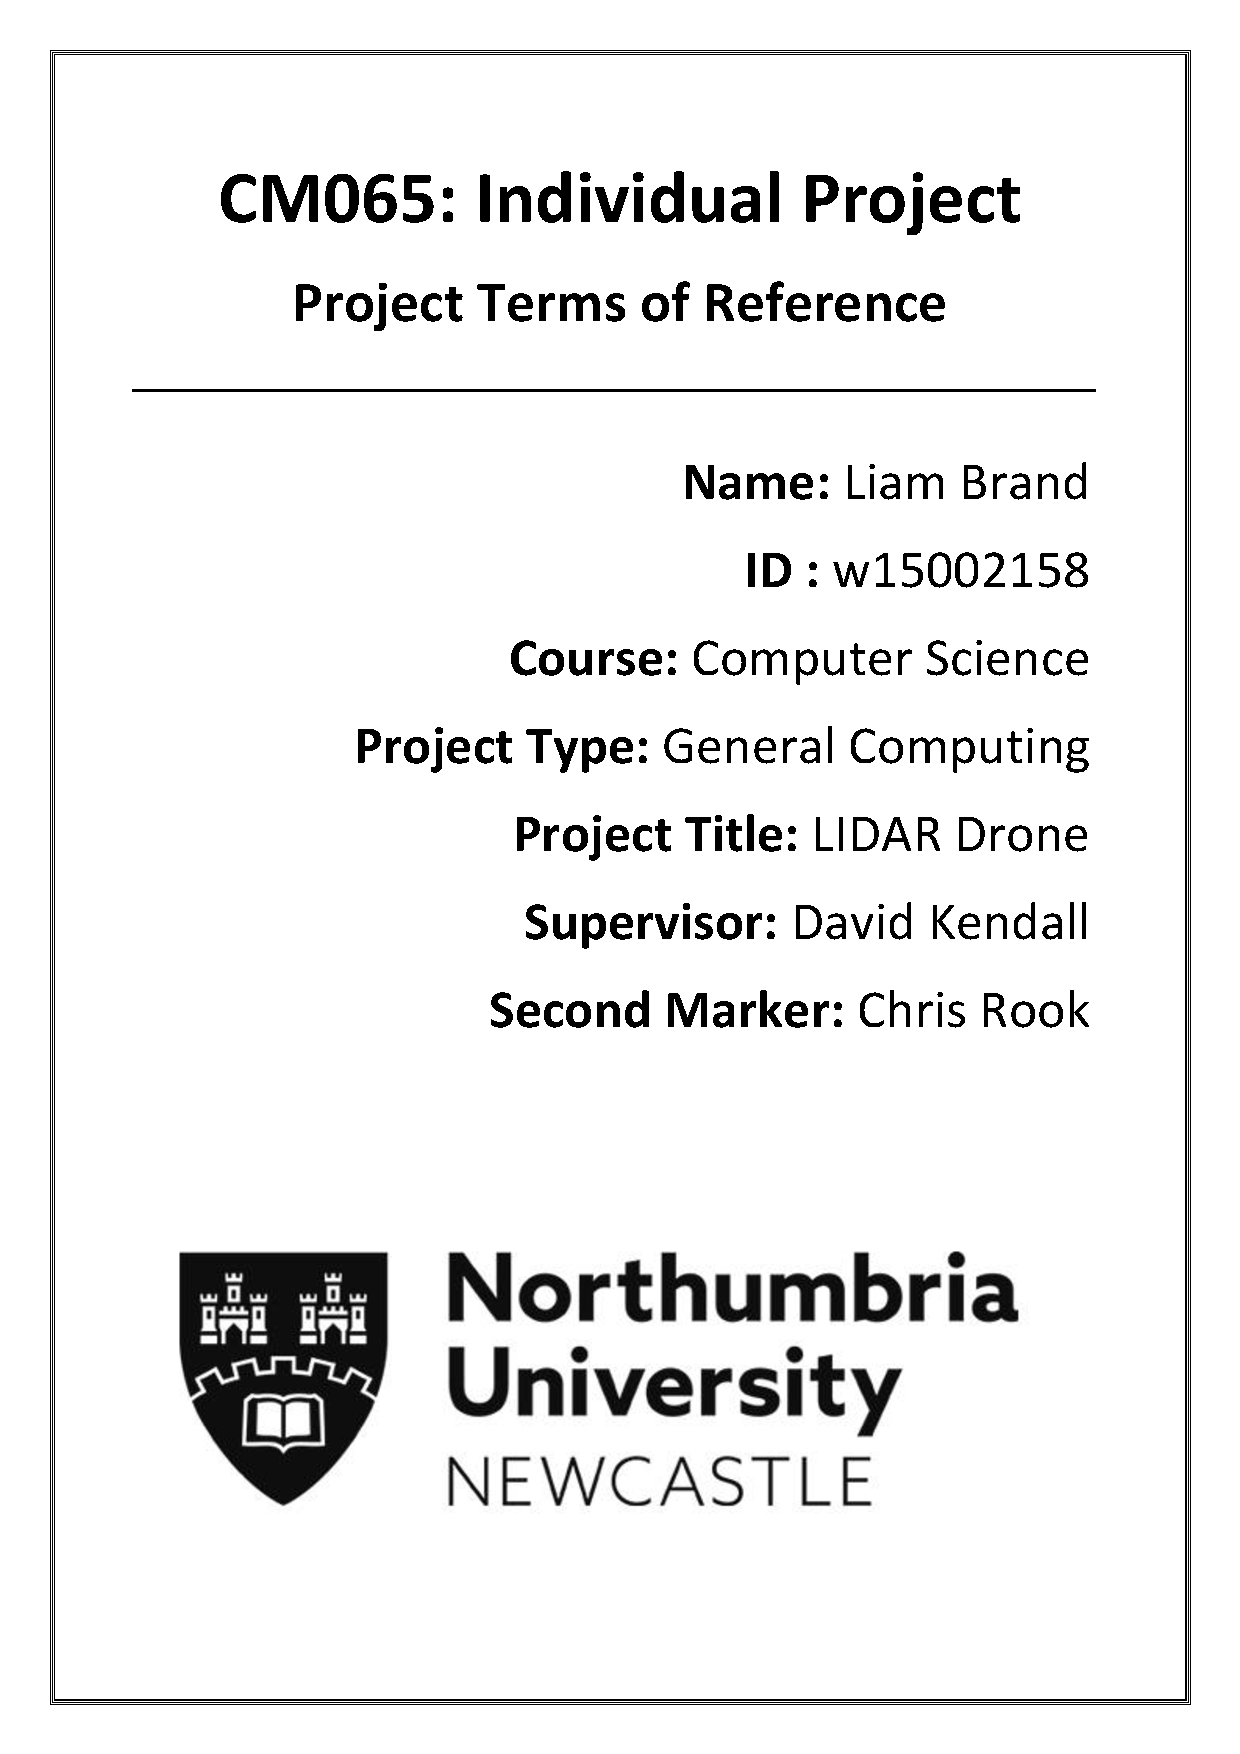
\includepdf[pages=-]{APPENDICES/TOR.pdf}
	\chapter{Program Code}
		\subsection{Robot Software}
			\subsubsection{main.cpp}
			\lstinputlisting{APPENDICES/main.cpp}
		\subsection{GUI}
			\subsubsection{mapgui.py}
			\lstinputlisting{APPENDICES/mapgui.py}
	\chapter{Testing}
	\begin{landscape}
	\label{testingappendices}
		\label{testing:testlogs}
					\begin{table}[h!]
						\centering
						\begin{tabular}{| l | l | l |} 
							\hline
							Printed Direction & Direction Moved In & Test Result  \\ [0.5ex] 
							\hline
							Right & Right & Pass   \\
							Left & Left & Pass   \\ 
							Forward & Forward & Pass   \\ 
							Left & Left & Pass   \\ 
							Right & Right & Pass   \\ 
							Forward & Forward & Pass   \\ 
							Right & Right & Pass   \\ 
							Left & Left & Pass   \\ 
							Backward & Backward & Pass   \\ 
							Forward & Forward & Pass   \\ 
							Backward & Backward & Pass   \\ 
							Left & Left & Pass   \\ 
							Right & Right & Pass   \\ 
							Right & Right & Pass  \\ 
							Backward & Backward & Pass   \\ 
							Forward & Forward & Pass   \\ 
							Forward & Forward & Pass  \\ 
							Backward & Backward & Pass  \\ 
							Right & Right & Pass   \\ 
							Forward & Forward & Pass   \\ 
							Backward & Backward & Pass   \\ [1ex] 
							\hline
						\end{tabular}	
					\caption{Movement Integration Tests}
					\label{table:movementtestsbasic}	
					\end{table}
				
					\begin{table}[h!]
						\centering
						\begin{tabular}{| p{2.5cm} | p{5cm} | p{4cm} | p{3cm} | p{1.5cm} |} 
							\hline
							Test & Test Purpose & Expected Result & Actual Result & Pass/Fail \\ [0.5ex] 
							\hline
							Begin sensor & Determine microcontroller's ability to start LIDAR sensor & Sensor starts spinning & As expected & Pass  \\
							
							Output reading & Determine ability to retrieve data from the LIDAR sensor & Terminal prints scan data & As expected & Pass \\
							 
							Stop sensor & Determine microcontroller's ability to stop LIDAR sensor & Sensor stops spinning & As expected & Pass   \\ [1ex] 
							\hline
						\end{tabular}	
					\caption{LIDAR Integration Tests}	
					\label{table:lidartestbasic}
					\end{table}
				
					\begin{table}[h!]
						\centering
						\begin{tabular}{| p{2.5cm} | p{5cm} | p{4cm} | p{3cm} | p{1.5cm} |} 
							\hline
							Test & Test Purpose & Expected Result & Actual Result & Pass/Fail \\ [0.5ex] 
							\hline
							File Creation & Ensure the robot can create files & File present on Micro SD-Card & As expected & Pass  \\
							
							Basic File Writing & Ensure created file contains data & File shouldn't be empty & As expected & Pass \\
							
							Accurate Data & Ensure written data is what the LIDAR has produced & File's data should match what has been output on the terminal & As expected & Pass \\ 
							
							Intense File Writing & See if the system can cope with writing many thousands of readings & File should contain more data, system task should still finish as normal & As expected & Pass \\
							[1ex] 
							\hline
						\end{tabular}
					\caption{File Writing Integration Tests}
					\label{table:filewritingtests}		
					\end{table}
				
					\begin{table}[h!]
						\centering
						\begin{tabular}{| p{2.5cm} | p{5cm} | p{4cm} | p{3cm} | p{1.5cm} |} 
							\hline
							Test & Test Purpose & Expected Result & Actual Result & Pass/Fail \\ [0.5ex] 
							\hline
							GUI Starts & Ensure the GUI starts properly & GUI will start up after being called from the command line & As expected & Pass  \\
							
							File Readings & Ensure the GUI can process the given file & GUI shouldn't encounter errors processing values from the file & As expected & Pass \\
							
							Basic Map Generated & Ensure a basic map can be generated  & GUI should display a map of the environment the robot mapped & Map was not accurate & Fail \\ 
							
							CSM Map Generated & Ensure the GUI can use CSM to generate a map  & GUI should output a map incorporating multiple scans & No such functionality implemented & Fail \\ [1ex] 
							\hline
						\end{tabular}
						\caption{Mapping Integration Tests}
						\label{table:mappingtests}		
					\end{table}
				
					\centering
					\begin{longtable}{| p{2.5cm} | p{5cm} | p{4cm} | p{4cm} | p{1.5cm} | p{2cm} |} 
						\caption{System Tests}
						\label{systemintergrationtestingtable} \\
						\hline
						Test & Test Purpose & Expected Result & Actual Result & Pass/Fail & Comments \\ [0.5ex] 
						\hline
						Drive Forward & The robot should move forwards during its operation & As expected & The robot moved forwards when it was switched on & Pass & Hardcoded movement  \\
	
						Drive Right & The robot should move right during its operation & The robot is able to move right & The robot couldn't move right & Fail &   \\
							
						Drive Left & The robot should move left during its operation & The robot is able to move left & The robot couldn't move left & Fail &   \\
						
						Obstacle Avoidance & The robot should navigate around obstacles during operation & The robot is able to avoid obstacles & The robot didn't detect obstacles & Fail &   \\
							
						Motor Obstructions & During the previous drive tests, there should be no obstructions to the motors from the robot's other components & As expected & The robot's motors didnt get blocked & Pass &   \\
						
						Power Failured & During the previous drive tests, there should be no power issues & Robot will complete operation without issue & Microcontroller battery's GND cable slips out & Fail &   \\
							
						Scanning & The robot should stop to scan & The robot stops and scans its environment & As predicteda & Pass &   \\ 
							
						Write Scan Data & Ensure the robot can write scanned data to the Micro SD-Card & The Micro SD-Card will contain a file with scan data & As expected & Pass & Plugged in and viewed with USB adapter  \\
							 
						Writing Duration & Ensure the robot writes data to the Micro-SD Card in a reasonable time  & Writing should be done in under ten seconds & As expected & Pass &   \\ 
							
						Generate Map & Using the robot's scan data, the GUI should produce a basic map & Map will be produced resembling the robot's environment & Map was produced but didn't resemble the environment & Fail &  \\ 
							
						Generate Map Without File & Make the GUI attempt to generate a map without an available file & GUI will catch and handle a runtime exception & As expected & Pass &  \\ 
							
						Map Multiple Areas & Mapping should work on multiple different environments & Each map will be accurate to the environment the robot was in & Maps didn't resemble the environment & Fail &  \\ 
							
						Repeated Mapping & Repeated maps of the same area should look similar & Map will be produced resembling the robot's environment & Maps didn't resemble the environment & Fail &  \\ 
							
						SLAM & The system should be capable of producing a dynamic map using multiple scans from different locations & The GUI creates a map from the robot's scan data & No such functionality & Fail &  \\ [1ex] 
							\hline
					\end{longtable}
			\end{landscape}			

		\section{Test Code}
		\label{testing:testcode}
			\subsection{Basic Movement Testing}
			\label{testcode:movementbasic}
			\begin{lstlisting}
while (true) {
	// Random number between 0 and 3
	int r = rand() % 4;
					
	if(r == 0) {
		pc.printf("Forward");
		goForward();
	}
					
	if(r == 1) {
		pc.printf("Right");
		goRight();
	}
					
	if(r == 2) {
		pc.printf("Back");
		goBackward();
	}
					
	if(r == 3) {
		pc.printf("Left");
		goLeft();
	}

	OSTimeDlyHMSM(0,0,3,0);
}
			\end{lstlisting}
			
			\subsection{LIDAR Testing}
			\label{testcode:observation1}
			\begin{lstlisting}
static void appTaskLidarTest(void *pdata) {
	dtr = 0;
	rplidar.begin(lidar_device);
	rplidar.startScan();
	struct RPLidarMeasurement measurement;
				
	while (true) {
		dtr = 1;
		rplidar.waitPoint();
		measurement = rplidar.getCurrentPoint();
		pc.printf("Distance: %f Angle:%f\n", measurement.angle, measurement.distance);
		dtr = 0;
		OSTimeDlyHMSM(0,0,1,0);
	}
}
			\end{lstlisting}
			
			\subsection{SDFileSystem Testing}
			\label{testcode:filewriting2}
			\begin{lstlisting}
dtr = 1;
rplidar.begin(lidar_device);
rplidar.startScan();
struct RPLidarMeasurement measurement;
				
static void writeTest() {
	struct RPLidarMeasurement measurement;

	// Create the readings file on the Micro SD-Card
	FILE *fp = fopen("/sd/readings.txt", "w");
					
	// Log if the file cannot be made
	if (fp == NULL) {
		pc.printf("Unable to access/create file \n");
	}

	for(int i = 0; i < 10; i++) {
		lidar.waitPoint();
		measurement = lidar.getCurrentPoint();
		pc.printf("Angle:%f Distance:%f\n", measurement.angle, measurement.distance);
		fprintf(fp, "%f %f\r\n", measurement.angle, measurement.distance);
	}
					
	// Close file
	fclose(fp);
}
			\end{lstlisting}
	
	\chapter{Hardware Documentation}
	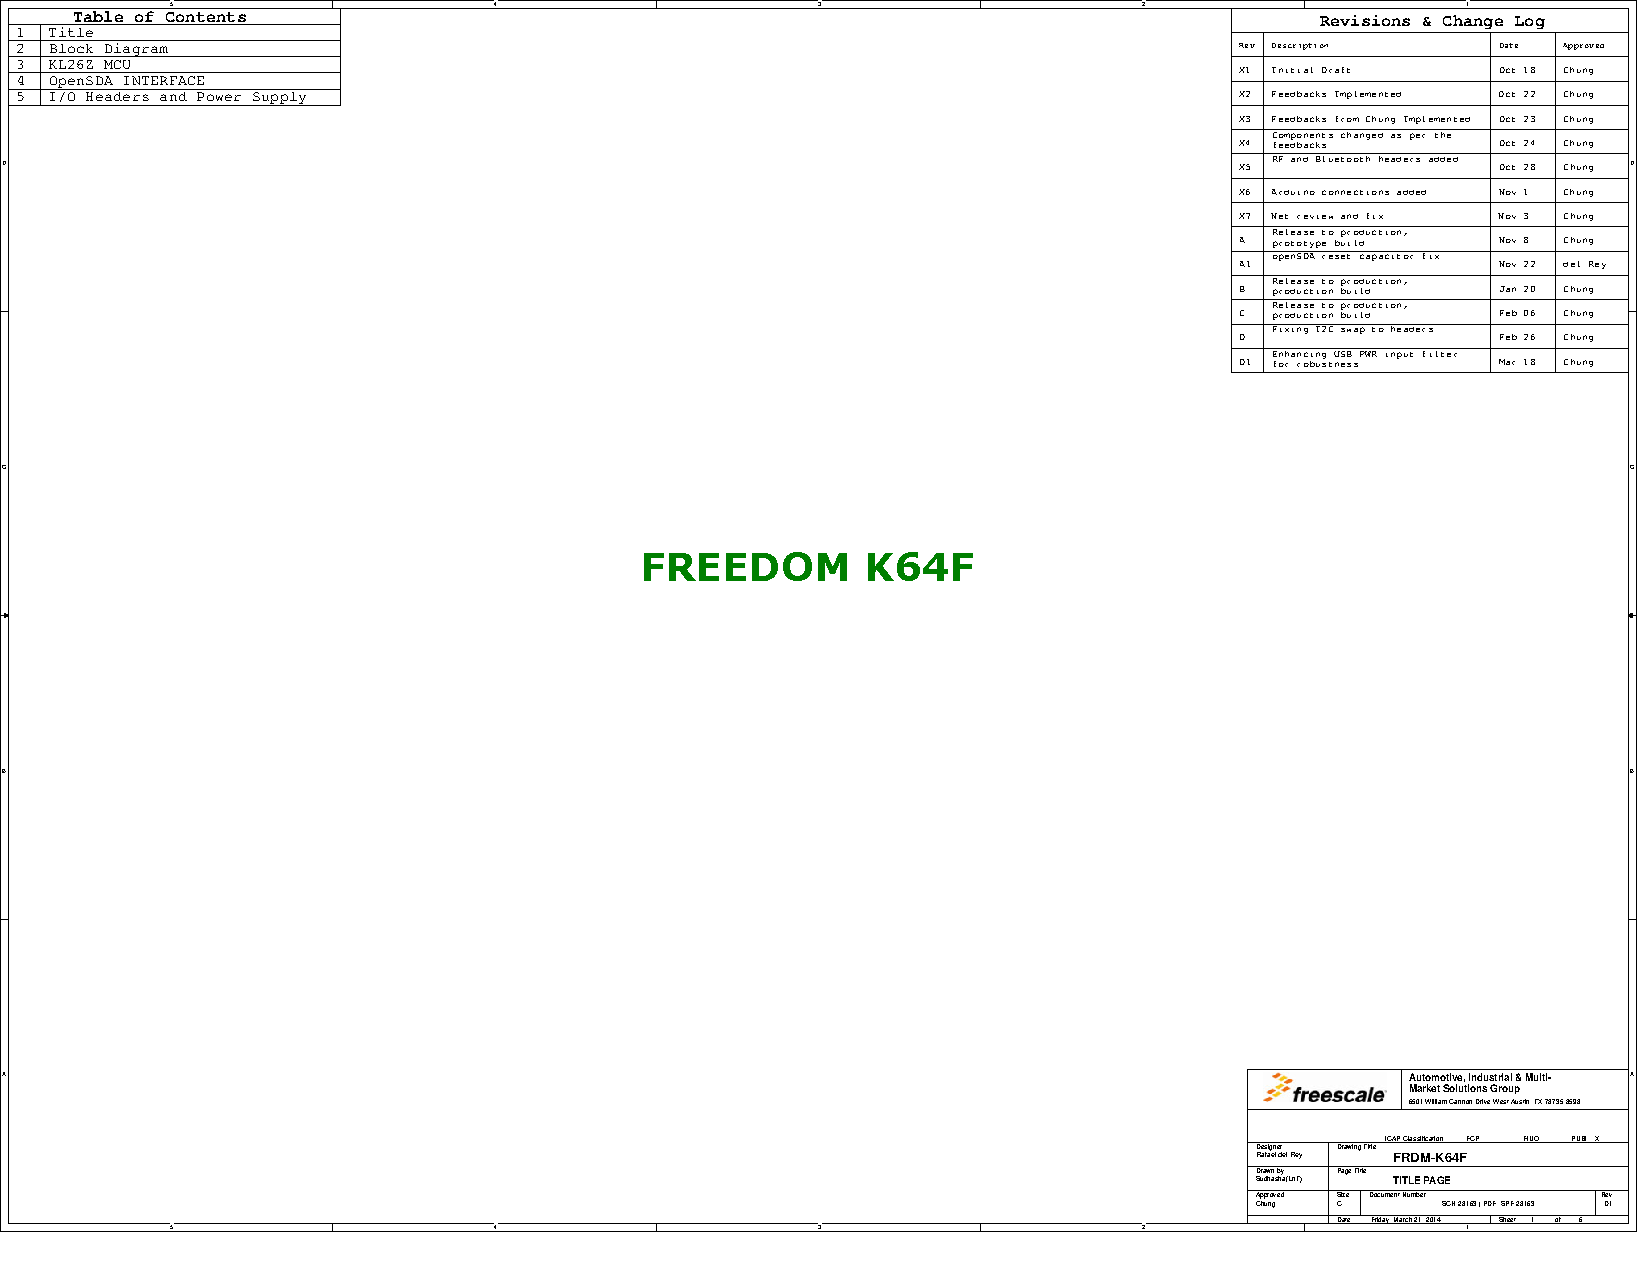
\includepdf[pages=-]{APPENDICES/k64fcircuitdiagram.pdf}
	\end{appendices}
			
